\documentclass{ctexart}
\usepackage[utf8]{inputenc}
\usepackage{graphicx}
\usepackage{amsmath}
\usepackage{amssymb}
\usepackage{enumitem}

\title{数值分析 - 第五次实验报告}
\author{强基数学2001班 樊睿 3200102142}
\date{December 11,2022}

\begin{document}

\maketitle

\begin{abstract}
本项目实现了对平面上 $n$ 个点用 $m$ 次多项式进行最小二乘拟合,并分析解决了一个实际例子。
\end{abstract}


\section{离散最小二乘拟合(DLS)}

\subsection{算法描述}
设计类 \verb|DLS| 对给定数据点 $\{(x_0,y_0),\dots,(x_{n-1},y_{n-1})\}$进行最小二乘拟合。

类的模板:\verb|template<class type>|

类的成员变量:
\begin{itemize}
\item 私有成员,\verb|Polynomial<type>| 类对象 $p$,拟合得到的多项式。多项式类的定义及实现详见第二章。
\end{itemize}

类的成员函数:
\begin{itemize}
\item 构造函数 \verb|DLS(vector<type>& x, vector<type>& y, int m, string method)|。\verb|x,y| 为数据集,\verb|m| 为拟合的多项式次数,\verb|method| 为拟合方法,可选 \verb|Normal|(正则方程组法)或 \verb|QR|(正交分解法)。
\item 公有函数 \verb|Polynomial<type> getpoly()|,获取构造出的多项式。
\end{itemize}

构造函数的算法步骤:

首先判断 \verb|method| 是正则方程组还是正交分解。

若是正则方程组:
\begin{itemize}
\item 预处理 $X_t=\sum_{i=0}^{n-1}x_i^t,0\leq t\leq 2m$。
\item 预处理 $Y_t=\sum_{i=0}^{n-1}x_y^ty,0\leq t\leq m$。
\item 则 $<x^i,x^j>=X_{i+j},<x^i,y>=Y_i(0\leq i\leq m,0\leq j\leq m)$。
\item 解线性方程组 $Ga=b$,其中 $G=(<x^i,x^j)_{(m+1)\times (m+1)}>,b=(<x^i,y>)_{m+1}$。
\item 返回多项式 $\sum_{i=0}^ma_ix^i$。
\end{itemize}

若是正交分解:
\begin{itemize}
\item 计算 $A=(x_i^j)_{n\times (m+1)}$。
\item 令 $b=(y_i)_{m+1}$。
\item 对 $A$ 进行 QR 分解 $A=QR$。
\item 解方程 $R_1a=Q^Tb$,其中 $R_1$ 为 $R$ 的前 $m+1$ 行。
\item 返回多项式 $\sum_{i=0}^ma_ix^i$。
\end{itemize}

注:QR分解及解方程组的部分在《数值代数》课程中已完整实现,封装在 Matrix 库(自编数值代数库)中的 \verb|QR_LS| 函数中,具体实现细节可参考库中代码。

\subsection{代码实现}
注释掉的部分是作答 B 题时需要的。
\begin{verbatim}
#include <bits/stdc++.h>
#include "../HW2/Polynomial.h"
#include "../Matrix.h"
using namespace std;

template<class type>
class DLS{
private:
    Polynomial <type> p;
public:
    DLS(vector<type>& x,vector<type>& y,int m,string method="Normal"){
        if(method!="Normal"&&method!="QR")throw "Invalid Method!";
        int n=x.size();
        p.resize(m+1);
        if(method=="Normal"){
            vector<vector<type>> px(2*m+1),py(m+1);
            vector<type> pxs(2*m+1),pys(m+1);
            Matrix<type> G(m+1,m+1);
            Colvec<type> c(m+1),sol;
            px[0].resize(n);
            for(int i=0;i<n;++i)px[0][i]=1;
            pxs[0]=n;
            for(int i=1;i<=2*m;++i){
                px[i].resize(n);
                for(int j=0;j<n;++j){
                    px[i][j]=px[i-1][j]*x[j];
                    pxs[i]+=px[i][j];
                }
            }
            py[0].resize(n);
            for(int i=0;i<n;++i)py[0][i]=y[i],pys[0]+=y[i];
            for(int i=1;i<=m;++i){
                py[i].resize(n);
                for(int j=0;j<n;++j){
                    py[i][j]=py[i-1][j]*x[j];
                    pys[i]+=py[i][j];
                }
            }
            for(int i=0;i<=m;++i)
                for(int j=0;j<=m;++j)
                    G[i][j]=pxs[i+j];
            for(int i=0;i<=m;++i)c[i]=pys[i];
            sol=Gauss_Improved_Solve(G,c);
            for(int i=0;i<=m;++i)p[i]=sol[i];
            /*答题用,使用时注释掉*/
            /*
            cout<<G<<endl;
            Symmetric_Diagnize(G);
            vector<type> eig(m+1);
            for(int i=0;i<=m;++i)eig[i]=fabs(G[i][i]);
            cout<<*max_element(eig.begin(),eig.end()) / *min_element(eig.begin(),eig.end())<<endl<<endl;
            */
            /**/
        }
        else if(method=="QR"){
            p.resize(m+1);
            Matrix<type> A(n,m+1);
            Colvec<type> b(n);
            for(int i=0;i<n;++i){
                A[i][0]=1;
                for(int j=1;j<=m;++j)A[i][j]=A[i][j-1]*x[i];
            }
            for(int i=0;i<n;++i)b[i]=y[i];
            pair<Matrix<type>,Colvec<type>> qr=QR(A);
            /*答题用,使用时注释掉*/
            /*
            for(int i=0;i<=m;++i){
                for(int j=0;j<i;++j)cout<<0<<' ';
                for(int j=i;j<=m;++j)cout<<qr.first[i][j]<<' ';
                cout<<'\n';
            }
            vector<type> eig(m+1);
            for(int i=0;i<=m;++i)eig[i]=fabs(qr.first[i][i]);
            cout<<*max_element(eig.begin(),eig.end()) / *min_element(eig.begin(),eig.end())<<endl<<endl;
            */
            /**/
            pair<Colvec<type>,type> sol=QR_LS(A,b);
            for(int i=0;i<=m;++i)p[i]=sol.first[i];
        }
    }
    Polynomial<type> getpoly(){return p;}
};
\end{verbatim}

附 Matrix 库中最小二乘代码。参考文献:《数值代数》徐树方著,第二版。

\begin{verbatim}
template <class T>
pair <Colvec <T>, T> house(const Colvec <T> & x) {
    int n = x.row();
    if (fabs(vert_inf(x)) < eps) return make_pair(e<T>(n, 0), 0);
    T S = 0;
    Colvec <T> v = x / vert_inf(x);
    for(int i = 1; i < n; ++ i) S += v[i] * v[i];
    if (S < eps) return make_pair(v, 0);
    T A = sqrt(S + v[0] * v[0]);
    if (v[0] <= 0) v[0] -= A;
    else v[0] = -S/(v[0] + A);
    T B = 2 * v[0] * v[0] / (S + v[0] * v[0]);
    return make_pair(v / v[0], B);
}

template <class T>
Matrix <T> house_trans(const Matrix <T> & a, const pair <Colvec <T>, T> & vb, bool type = 0) {
    if (!type) {
        Colvec <T> v = vb.first;
        v[0] = 1;
        return a - v * ~(~a * v * vb.second);
    } else {
        Colvec <T> v = vb.first;
        v[0] = 1;
        return a - a * (vb.second * v) * ~v;
    }
}

template <class T>
pair <Matrix <T>, Colvec<T> > QR(const Matrix <T> & a) {
    Matrix <T> b = a;
    int m = a.row(), n = a.col();
    Colvec <T> d(n);
    pair <Colvec <T>, T> h;
    for(int k = 0; k < n; ++ k){
        h = house(split(b, k, k, m));
        update(b, house_trans(split(b, k, m, k, n), h), k, m, k, n);
        d[k] = h.second;
        for(int i = k+1; i < m; ++ i) b[i][k] = h.first[i-k];
    }
    return make_pair(b, d);
}

template <class T>
pair <Colvec <T>, T> QR_LS(const Matrix <T> & a, const Colvec <T> & b) {
    int m = a.row(), n = a.col();
    pair <Matrix <T>, Colvec <T> > qr = QR(a);
    Colvec <T> c = b;
    for(int k = 0; k < n; ++ k)
        update(c, (Colvec <T>)house_trans(split(c, k, m), make_pair(split(qr.first, k, k, m), qr.second[k])), k, m);
    Colvec <T> x = BSP(split(qr.first, 0, n, 0, n), split(c, 0, n));
    T res = vert_2(split(c, n, m));
    return make_pair(x, res);
}
\end{verbatim}

\section{问题求解}

\begin{verbatim}
#include<bits/stdc++.h>
#include "DLS.h"
using namespace std;
int main(){
    vector<double> x({0,0.5,1,1.5,2,2.5,3,3.5,4,4.5,5,5.5,6,6.5,7,7.5,8,8.5,9,9.5,10});
    vector<double> y({2.9,2.7,4.8,5.3,7.1,7.6,7.7,7.6,9.4,9.0,9.6,10.0,10.2,9.7,8.3,8.4,9.0,8.3,6.6,6.7,4.1});
    DLS<double> dlsn(x,y,2);
    DLS<double> dlsq(x,y,2,"QR");
    cout<<dlsn.getpoly()<<endl;
    cout<<dlsq.getpoly()<<endl;
}
\end{verbatim}

对于 B 题中的数据,两种方法输出了同样的拟合多项式 $2.17572 +2.67041x -0.238444x^2$。

最小二乘曲线和数据点的分布如下:

\begin{figure}[h]
    \begin{minipage}{4cm}
	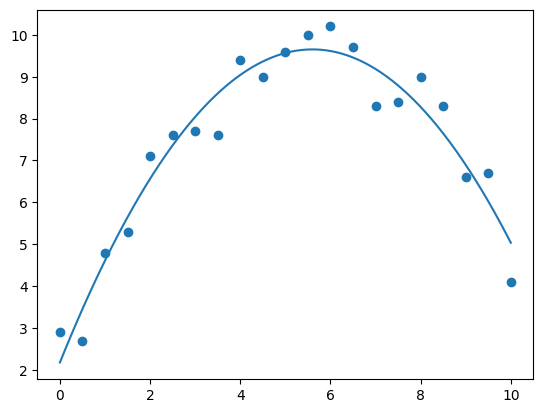
\includegraphics[width = 12cm, height = 8cm]{1.png}
	\label{fig1}
	\end{minipage}
\end{figure}

附作图程序:

\begin{verbatim}
import matplotlib.pyplot as plt
import numpy as np

def f(x):
    return 2.17572 +2.67041*x -0.238444*x**2

xs = [0,0.5,1,1.5,2,2.5,3,3.5,4,4.5,5,5.5,6,6.5,7,7.5,8,8.5,9,9.5,10]
ys = [2.9,2.7,4.8,5.3,7.1,7.6,7.7,7.6,9.4,9.0,9.6,10.0,10.2,9.7,8.3,8.4,9.0,8.3,6.6,6.7,4.1]
plt.scatter(xs, ys)

x = np.linspace(0, 10, 1000)
y = [f(t) for t in x]
plt.plot(x, y)

plt.show()
\end{verbatim}

正则方程组中,
\begin{equation}
G=
\begin{bmatrix}
21 & 105 & 717.5 \\
105 & 717.5 & 5512.5 \\
717.5 & 5512.5 & 45166.6 \\
\end{bmatrix}
\end{equation}

用 QR 方法(详见 \verb|Matrix.h|)求得特征值为 $45851,761.682,707.566$,二范数下条件数为 $64.8011$。

正交分解法中,

\begin{equation}
R_1=
\begin{bmatrix}
4.58258 & 22.9129 & 156.571 \\
0 & 13.8744 & 138.744 \\
0 & 0 & 37.4438 \\
\end{bmatrix}
\end{equation}

$R_1$ 是上三角阵,因此特征值就是对角元。为 $37.4438,13.8744,4.58258$,二范数下条件数为 $8.17092$。

矩阵的条件数反映了方程组的稳定性,进而反映了算法的稳定性。因此,正交分解的稳定性比正则化方程组要好。

\end{document}